% XCircuit output "linear_sim_s_domain.tex" for LaTeX input from linear_sim_s_domain.ps
\def\putbox#1#2#3{\makebox[0in][l]{\makebox[#1][l]{}\raisebox{\baselineskip}[0in][0in]{\raisebox{#2}[0in][0in]{#3}}}}
\def\rightbox#1{\makebox[0in][r]{#1}}
\def\centbox#1{\makebox[0in]{#1}}
\def\topbox#1{\raisebox{-\baselineskip}[0in][0in]{#1}}
\def\midbox#1{\raisebox{-0.5\baselineskip}[0in][0in]{#1}}
\begin{flushleft}
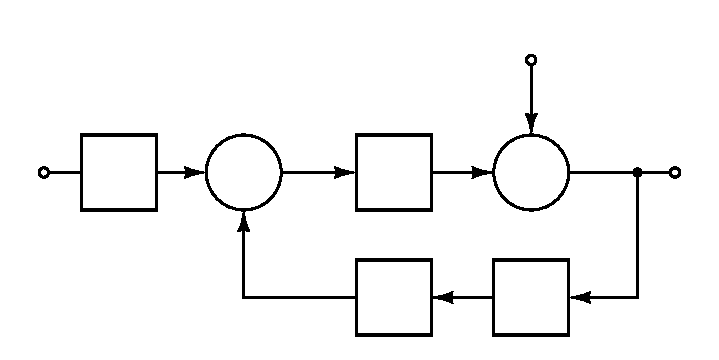
\epsfig{file=linear_sim_s_domain.ps}\\
% translate x=752 y=400 scale 0.38
\putbox{1.51in}{1.18in}{\centbox{\midbox{$\displaystyle\sum$}}}%
\putbox{4.39in}{1.35in}{\centbox{\midbox{$Y(s)$}}}%
\putbox{0.18in}{1.35in}{\centbox{\midbox{$X(s)$}}}%
\putbox{0.68in}{1.18in}{\centbox{\midbox{$F(s)$}}}%
\putbox{2.51in}{1.18in}{\centbox{\midbox{$G(s)$}}}%
\putbox{2.51in}{0.35in}{\centbox{\midbox{$H(s)$}}}%
\putbox{1.39in}{0.85in}{\centbox{\midbox{$-$}}}%
\putbox{3.43in}{2.10in}{\centbox{\midbox{$E(s)$}}}%
\putbox{3.43in}{1.18in}{\centbox{\midbox{$\displaystyle\sum$}}}%
\putbox{3.43in}{0.35in}{\centbox{\midbox{$t_D$}}}%
\end{flushleft}
